\section{Persistent Data Management}
Data of all entities in the \texttt{DriveIT System} are stored persistently to avoid data loss if the system crashes, and to ensure that users can expect to resume work from the point where they last left.
The \texttt{Persistent Storage} subsystem stores this data using a \textit{DBMS}\footnote{\url{http://en.wikipedia.org/wiki/DBMS}} hosted online - more specifically in a Microsoft SQL database.\\

It stores the following entities:
\begin{itemize}
	\item \textbf{Car:} Representing a used car. \texttt{Car}s are created, read, modified, and deleted by subsystems in the \texttt{DriveIT System}.\\
	\texttt{Car}s have many attributes, all describing the properties of the used car. \texttt{Car}s are referenced in many other entities in the storage system, but do not reference other entities themselves.
	\item \textbf{Customer:} Representing a potential buyer of car(s). \texttt{Customer}s are read by some parts of the system, but only modified and deleted in certain authorized instances.\\
	\texttt{Customer}s have few attributes describing the person acting as the customer. \texttt{Customer}s are referenced in some entities in the storage system, but do not reference other entities themselves.
	\item \textbf{Employee:} Representing a salesman of cars. \texttt{Employee}s are read by some parts of the system, but only modified and deleted in certain authorized instances.\\
	\texttt{Employee}s have few attributes describing the person selling cars. \texttt{Employee}s are referenced in some entities in the system, but do not reference other entities themselves.
	\item \textbf{Sale:} Representing a sale of a car. \texttt{Sale}s are only created, read, modified, and deleted in certain authorized instances.\\
	\texttt{Sale}s have few attributes describing the specific sale, but mainly reference other entities. A given \texttt{Sale} references an \texttt{Employee}, a \texttt{Car} and a \texttt{Customer}.
	\item \textbf{Comment:} Representing a comment on a car. \texttt{Comment}s are read by some parts of the system, but only modified and deleted in certain authorized instances.\\
	\texttt{Comment}s have few attributes describing the specific comment, but mainly reference other entities. A given \texttt{Comment} references a \texttt{Car} and a \texttt{Customer}.
	\item \textbf{ContactRequest:} Representing a customer's request for contact about a car which can be followed up by an employee. \texttt{ContactRequest}s are only created, read, updated, and deleted in certain authorized instances.\\
	\texttt{ContactRequest}s have one attribute describing the specific request, but mainly reference other entities. A given \texttt{ContactRequest} references a \texttt{Car}, a \texttt{Customer} and optionally an \texttt{Employee}.
\end{itemize}
Figure \ref{fig:persistentDataModel} shows all entities with their respective attributes.
	\begin{figure}[H]
		\centering
		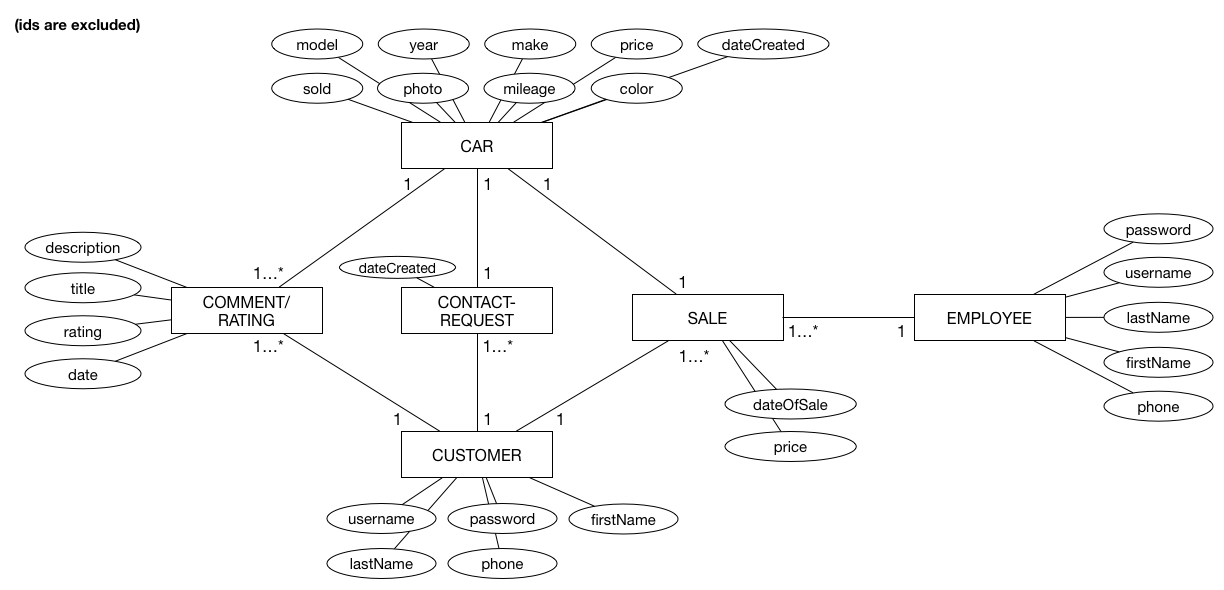
\includegraphics[width=\textwidth]{Figures/PersistentDataModel}\\
		% place the figure in the Figures folder (located with the main file)
		% you need to fix the scale a few times to get it right, but latex does not compress so one can always zoom in to see details.
		\caption{The Persistent Data Model.}
		\label{fig:persistentDataModel}
	\end{figure}